\documentclass[../main.tex]{subfiles}
\graphicspath{{\subfix{../images/}}}

\begin{document}
	
\chapter{Methodology}
\section{Introduction}

To analyze the performance of different support structures created using topology optimization, a comparison study was made in which parts created by additive manufacturing were paired with different support structures. This study assumed that different structures will conduct heat energy differently, and thus some topologies might be more effective in removing heat faster from each material layer as it is being processed. This increased thermal conduction would then result in less overall thermal deformation, as the manufactured component would expand less due to the decreased time in high temperatures. 

This section will explain the full process taken to run the simulations and analyze the data. An overview of the process can be seen in Figure~\ref{fig:process_diagram}. The process starts from the creation of the CAD for the manufactured components, followed by the design and CAD creation of the support structures. The components and the support structures are then merged, and imported into the additive manufacturing software to simulate the results of manufacture. The results from the manufacturing simulation are then analyzed by means of graphs and statistical methods. 

\begin{figure}
  \begin{center}
    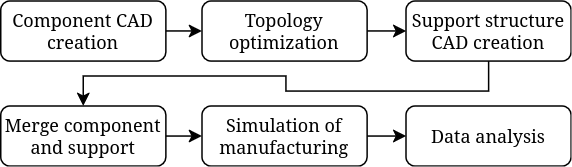
\includegraphics[width=0.95\textwidth]{process_diagram.png}
  \end{center}
  \caption{Process diagram.}\label{fig:process_diagram}
\end{figure}

The subsequent sections explain in detail each stage of this process.

\section{Component CAD creation}

\subsection{Simple geometry}

The components with simple geometries utilized in this study consist of a cube, three triangular
components with different slopes, and three cylindrical components with different values of
curvature. To reiterate, these components have the same dimensions that were used in the study of lattice
support structure performance by Peishu \cite{peishu_thesis}. All the CAD models
used for the simple geometry study were created using FreeCAD, an open-source CAD software. All the components were expoerted as .STEP files, and then they were merged with their corresponding support structures using the software nTop. 

\begin{itemize}
  \item A cube with side length of 30 mm (Figure \ref{fig:cube}).
  \item Three triangular components with varying slopes. All triangular components have a base of 30 x 30 $mm^2$, with slopes of 15 \degree, 30  \degree and 45 \degree. The measurements are shown in figure. \missingfigure{measurements of triangles.}
  \item \todo{Add cylinders here}
\end{itemize}

\begin{figure}
	\begin{center}
		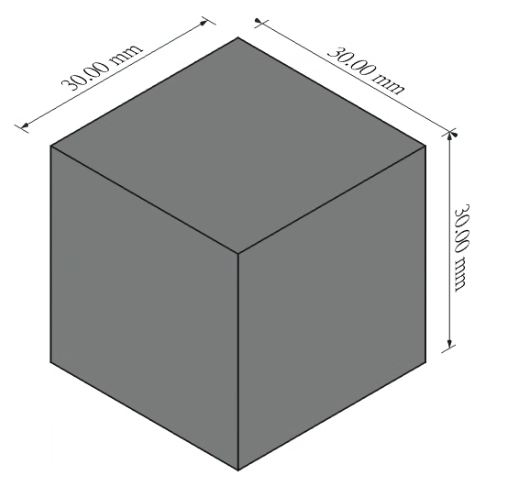
\includegraphics[width=0.45\textwidth]{cube.png}
	\end{center}
	\caption{Dimensions of cube component.}\label{fig:cube}
\end{figure}

\todo{Add figure of cylinders}

\subsection{Femoral component}

\missingfigure{Figure of cylindrical geometry}

\section{Support structure creation}

The supporting structures of the components were created using the method of topology optimization. The design was implemented using the topology optimization module of COMSOL Multiphysics 6.2.  

The steps for creating a valid topology optimization model are: determine the design volume, choose a suitable mathematical model for the behavior of the material within the design volume, choose the objective functions and decide what constraints need to the material within the volume be applied to the design volume. The following section explains all of these steps in detail.

\subsection{Design domain}

\todo{need to expand on this and make it better. need to get dimesions of components}

\subsubsection{Simple geometry design domain}

The design domain for the simple geometry components consists of the volume between the bottom face of each component and the base plate. For the cube, the design domain ends up being a rectangular prism with dimensions 10 cm x 30 cm x 30 cm. For the triangles, the design domain consists of different triangular spaces with a square base, shown in figures \missingfigure{figures of triangular domain}. \todo{Add here the cylindrical component geometry}.

Since all of these components can be generated by the drawing their profile on a plane and extruding it in a direction perpendicular to the plane, the design domain utilized in the topology optimization model is also a 2D model. This grants the benefit of faster computation, and thus the supporting structure is created by first finding the planar topology and also extruding it in a perpendicular direction. 

\subsubsection{Femoral component design domain}

\subsection{Mathematical model}

The mathematical models consists of the governing equations used to describe the physics of the system and the constraints imposed on the model, as well as the objective function that needs to be minimized. 

For this system, the most appropriate objective function would be the maximization of thermal conductivity; in order to minimize the thermal deformation of the manufactured component, it is imperative to transfer heat away from it as fast as possible. The physical equation describing the thermal conduction of a material is given by Fourier's Law, which can be expressed as:

\begin{equation}
  \label{eq:Fourier Law}
  q = -k \nabla T
\end{equation}

where q is the heat conduction through the material, k is the material's thermal conductivity and $\nabla T$ is the thermal gradient. 

For this study, the only constraint applied on the system was the volume fraction. Volume fraction speficies the maximum amount of volume that the designed topology should take from the design domain. The volume fractions utilized were 50\% and 75\%.

\todo{Write down equation of thermal conductivity for top optimiation domain here.}

\subsection{Objective functions}

An additional objective function to be considered would be the deformation of the supporting structure as well. If the supporting structure is composed of very thin segments, there is a high possiblity that the structure might buckle, which would add significant geometric errors to the component. In the worst case scenario, the structure itself would collapse, causing the entire manufacturing process to fail. In order to avoid this, it is necessary to limit the amount of deformation that is allowed in the support structure. This can be achieved by utilizing an aditional objective function of structural compliance minimization. We define structural compliance as the amount of energy stored in the deformation of material. Minimizing this stored energy is thus equivalent to minimizing the deformation. \todo{probably want to add a reference to this somewhere.} Therefore, the second objective function of minimization of structural compliance is also used in the topology optimization model.as heat passes into the support structure from the bottom of the manufactured component,

\todo{Write equation of compliance here}

\todo{Merge them together to get the final objective function. Explain about the weights.}

The next step is applying certain constriants on the system. For this study, we are mostly concerned with the principal constrain is the volume fraction, which is the maximum amount of volume that the topology can cover within the design domain. This criteria is chosen because we seek to use less material for the supporting structure, as long as we can maintain the total deformation of the manufacturing componont beneath a threshold. For the model in COMSOL, the values of volume fraction = 0.5 and volume fraction = 0.75 were used.

\subsection{COMSOL implementation}

\subsubsection{Mesh}

\subsubsection{Physical parameters}

\subsubsection{Simulation itself}

\todo{Talk about Helmholtz filter}

As discussed in the previous chapter, Helmholtz filters are frequently used in topology optimization studies to avoid chattering designs. 

\todo{Hyperbolic tangent}

\section{Component and support structure merging}

\subsection{CAD for support structure}

This section talks about how FreeCAD was used to create the support structure once the pictures of the topolgies have been obtained.

\subsection{Merging of part with support structure}

Once the CAD file of the component and the support structure has been built, it is necessary to merge them together and import them into Simufact to undergo simulation of the manufacturing process. The software used for blending the component and its support structure is nTop \todo{add version here}. nTop's interface makes it very easy to merge the part, and also allows to blend the support structure and the component, which effectively creates a fillet between the nodes of both components to allow for a smooth transition between bodies. Of course, blending the component and the support structure in this manner would not give any benefit in a real manufacturing process, as the structure and the component would not be able to be separated easily. NEvertheless, this blend radius is beneficial for the simulation since it was observed that a direct union and import of the support structure + component in Simufact resulted in having very small gaps between the two pieces, resulting in a non manifold geometry that would cause the finite element model to have gaps between some of its nodes. 

\missingfigure{add figure of error / warning from Simufact due to import of structure with gaps. Two figures should suffice here.}


\section{Simulation of manufacturing process}


The software utilized to simulate the manufacturing process is Simufact Additive version 2023.2. Simufact Additive is capable of simulation building process of additive manufacturing components, and coupling thermal and stress physics to predict the temperature values of the component throughout the building process and the total stresses, strains and deformations resulting from the manufacturing process. 

In order to set up Simufact correctly, the building process and the building space geometry must be specified before each simulation. The building parameters and building geometries used in this study are the same that were used in the analysis of thermal deformation using lattice support structures done by Peihsy and al. \todo{add reference here}

\subsection{Simufact simulation parameters and voxelization}

\todo{add that thermomechanical process was used and explain what it is.}

After the component and the support structures were merged, they were imported into Simufact. It is during this step that all the factors related to the simulation are set, which include the machine properties, material properties, and build parameters. As mentioned previously, these were chosen to be identical to the study of PeiHsu to ensure that the results of this study could be compared to the results of that one. 

The first parameter to be chosen is the process properties, which determines the physics that Simufact takes into consideration to run the simulation. Simufact provides three different types of processes: mechanical, thermal, and thermomechanical. As stated in the Simufact manual \todo{insert reference to manual here}, mechanical provides a fast mechanical analysis that only uses inherent strains as the main input. This type of analysis does not take into consideration the temperature fields during the building process. The thermal process on the other hand only considers the thermal behaviour of the components, and the temperature field of the support structures, components and base can be analyzed. The thermomechanical process couples the stress and thermal analyses, and allows for the prediction of temperature, distortions and stresses of the part. This latter process is the one used in this study.

After choosing the process property, the machine parameters must be specified. This includes the machine build plate geometry and the laser parameters. The machine build plate chosen was a circular plate with an 80 mm radius. The build space dimensions consists of a space of 160 mm in all three x-y-z directions. As for the laser parameters, the simulations were carried out with one laser with a maximum laser power of 500 W and a maximum laser speed of 2000 mm / s, an efficiency of 25 percent, and a beam width of 25 mm. All of these parameters are summarized in the table \todo{add the table of building parameters here.}

The building parameters for the process need also to be set. These include material layer parameters and any thermal parameters and temperature specifications for the build environment and base plate. The powder layer thickness was chosen to be 0.03 mm, with a recoater time of 10 s. The powder initial temperature was set to 25 \degree Celcius, with an initial base temperature of 200 degrees. \todo{explain why base plate temeprature might be used in practice, might want to add reference to 10.3390/thermo4010005}

\todo{Need to add exposure time, exposure energy fraction, and volumetric expansion factors here. Need to refer to Comsol documentation to explain what these are and how they influence the results.}

\todo{Need to say that no calibration was done. Explain why calibration is necessary for the manufacture of parts, but also explain the reason no calibration was done here.}

\todo{Explain what this is and how it is done, and what the purpose of this is.}

\subsection{Convergence analysis}

To make sure that the results of the simulation would not depend on the voxel density of the 

\section{Data collection and organization}

\textit{This section will detail how I collected the data from Simufact and what software and methods I used to organize it an analyze it. The actual results will go in the following chapter, aptly named results, duh}

\listoftodos

\end{document}
